%!TEX program = xelatex
% 完整编译方法 1 pdflatex -> bibtex -> pdflatex -> pdflatex
% 完整编译方法 2: xelatex -> bibtex -> xelatex -> xelatex
\documentclass[lang=cn,11pt]{elegantpaper}

\title{实验5:路由器的配置实验报告}
\author{\href{https://github.com/Jack-Lio}{李伟}}

\institute{1711350   计算机科学与技术一班}

% 不需要版本信息,直接注释即可
%\version{0.07}
% 不需要时间信息的话,需要把 \today 删除。
\date{\today}


% 如果想修改参考文献样式,请把这行注释掉
\usepackage[authoryear]{gbt7714}  % 国标

\begin{document}

\maketitle

\begin{abstract}
\noindent 路由的配置和维护是网络管理员的一项重要任务。路由的正确配置是保证互联网畅通的首要条件。同时,为了深入理解互联网的工作机理,
本实验通过在windows虚拟机以及\lstinline{Cisco Packet Tracer}仿真环境中进行路由的配置工作,实现构建一个小型的网络互联环境,了解路由配置的相关知识和具体细节,进一步理解IP地址的分配和工作原理。
\keywords{路由器配置,静态路由,\lstinline{RIP},\lstinline{CISCO Packet Tracer}}
\end{abstract}


\section{实验要求}

本实验分为两个部分,分别要求在4台\lstinline{Windows Server 2003}虚拟机上进行路由器网络的配置以及在\lstinline{Cisco Packet Tracer}仿真环境下进行路由器网络的配置,配置实现的网络结构能够满足以下的检查条件:
\begin{itemize}
	\item 两个实验中路由器的任何一台主机均可以通过\lstinline{ping}命令或者\lstinline{tracert}命令连通至另外一台主机,并且输出正确。
	\item 在配置主机IP地址的过程中使用不同的网络前缀实现,同时需要实现静态路由和RIP动态路由选择协议的配置。
\end{itemize}

\section{实验环境}
\subsection{虚拟机路由配置}
\begin{itemize}
	\item 虚拟机系统环境 windows 2003 server
	\item 虚拟机运行环境 windows 7
	\item 虚拟机配置 1G内存 单核CPU
\end{itemize}
\subsection{仿真环境路由配置}
\begin{itemize}
	\item 操作系统环境 windows 10 
	\item 仿真环境 Cisco Packet Tracer 7.1
\end{itemize}

\section{实验具体步骤}
本次实验的实现分为两个大的部分,需要分别的四台\text{windows 2003 server}上以及\text{Cisco Packet Tracer}上实现路由配置,同时对每一种环境均需要实现静态路由和动态路由两种方式。具体的实现步骤如下所述:
\subsection{虚拟机路由配置}
\subsubsection{IP地址配置}
首先,考虑虚拟机的静态路由配置实现,通过\text{windows 2003 server}提供的路由和远程访问程序,可以便捷的设置每一台主机相应网卡的IP地址配置,在本次实验中四台虚拟机(两台作为路由机器,两台作为终端机器)的IP地址配置如\figref{fig:tuopu}所示:
\begin{figure}[htbp]
	\centering
	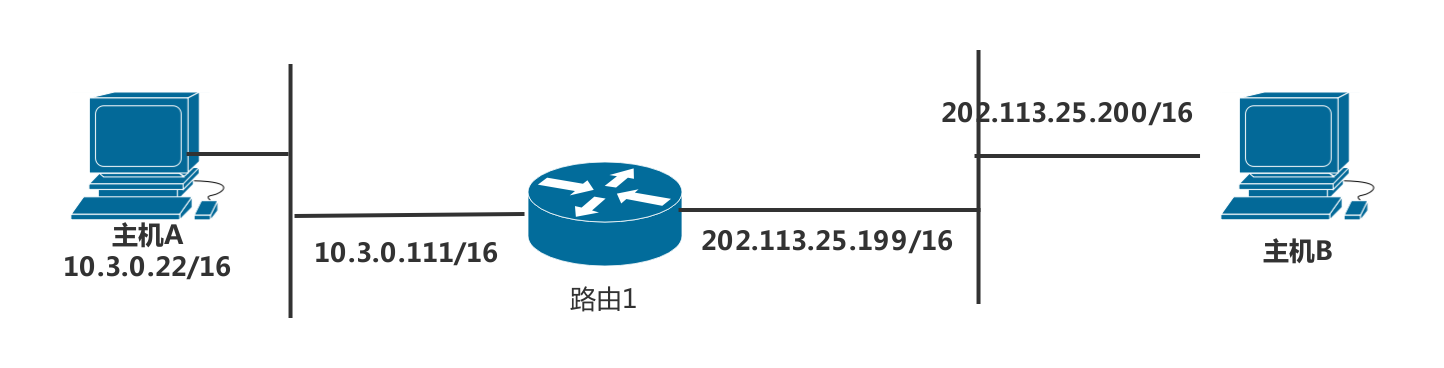
\includegraphics[width=0.6\textwidth]{互联网拓扑图}
	\caption{虚拟机互联网拓扑图结构 \label{fig:tuopu}}
\end{figure}
设置虚拟机的IP地址的步骤为:选择“路由与远程访问”的本地接口,选择“常规”,在界面中可以看到两个本地连接,分别对应虚拟机的两个网卡,在本次实验中,主要是基于单网卡双IP的方式,所以只需要选择一张网卡,为其添加两个IP即可实现路由器的IP地址配置\footnote{之所以选择单网卡双IP的方案,是因为本次实验需要实现动态和静态两种路由配置,单网卡双IP的方式,四台机器八个网卡正好够用。},可以通过双击“本地连接”打开配置窗口,进行IP地址的添加,如果要添加多个IP则需要打开配置的高级选项功能。

需要注意的是,作为终端机使用的主机A和主机B需要在设置IP地址的同时,设置好对应的默认路由。
\subsubsection{路由器静态路由配置}
配置好虚拟主机的IP地址之后,开始为路由器R1和R2配置静态路由,配置方式可以是命令行配置,也可以是通过“路由与远程访问”程序实现,在这里以后一种方式说明,“程序与远程访问”界面如\figref{fig:jiemian}所示:
\begin{figure}[htbp]
	\centering
	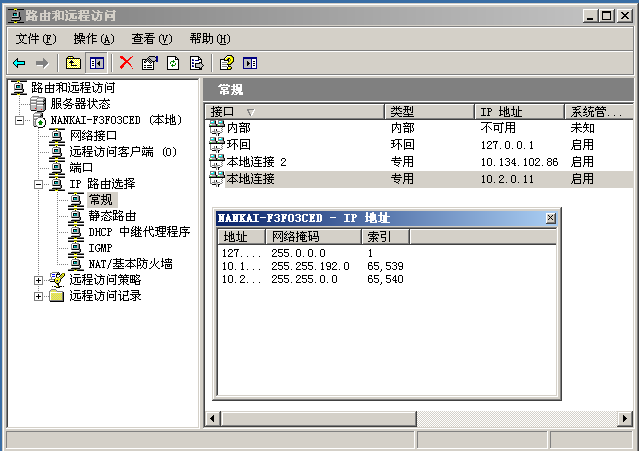
\includegraphics[width=0.6\textwidth]{ipset3}
	\caption{程序与远程访问界面截图演示\label{fig:jiemian}}
\end{figure}
从截图\figref{fig:jiemian}可以看到静态路由的选项,打开后在空白界面右键选择“新建静态路由”即可选择为相应的网卡连接添加静态路由,为\figref{fig:tuopu}中的R1与R2添加静态路由后的“程序与远程访问”界面\figref{fig:static1}、\figref{fig:static2}所示:

\begin{figure}[htbp]
	\begin{minipage}[t]{0.48\textwidth}
	\centering
	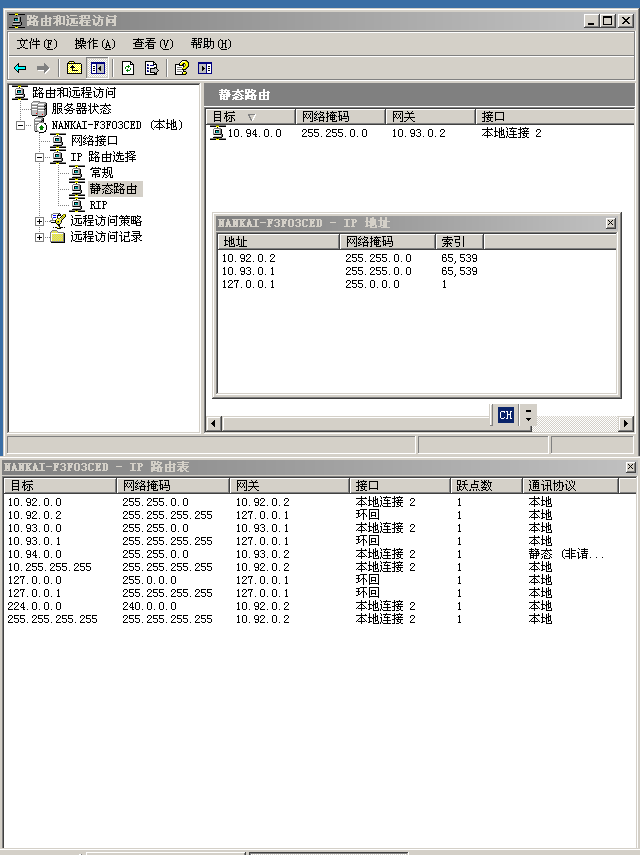
\includegraphics[width=0.6\textwidth]{s2}
	\caption{R1添加到网络\text{10.94.0.0}的静态路由\label{fig:static1}}
	\end{minipage}
\begin{minipage}[t]{0.48\textwidth}
	\centering
	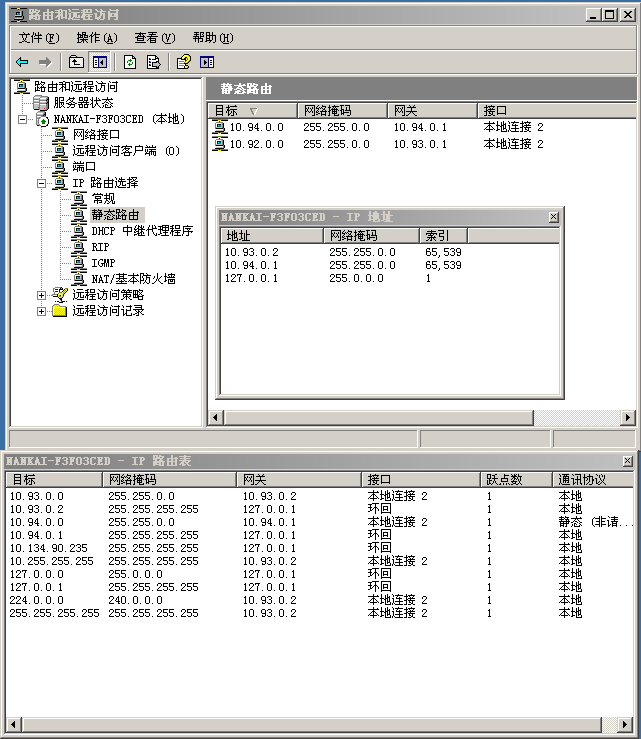
\includegraphics[width=0.7\textwidth]{z3t}
	\caption{R2添加到网络\text{10.92.0.0}的静态路由 \label{fig:static2}}
\end{minipage}
\end{figure}

\subsubsection{RIP路由协议配置}
除了通过静态路由配置之外,还可以通过添加RIP动态路由协议实现自动的路由配置,配置的方法为选择一个网卡连接,右击之后选择添加协议,然后选择RIP version2,之后在左侧的导航栏中会出现RIP的导航项,点击进入后,在空白处右击新建一个RIP(给对应的网卡)。为R1与R2设置RIP协议之后的界面如\figref{fig:rip1}、\figref{fig:rip2}所示:
\begin{figure}[htbp]
	\begin{minipage}[t]{0.48\textwidth}
		\centering
		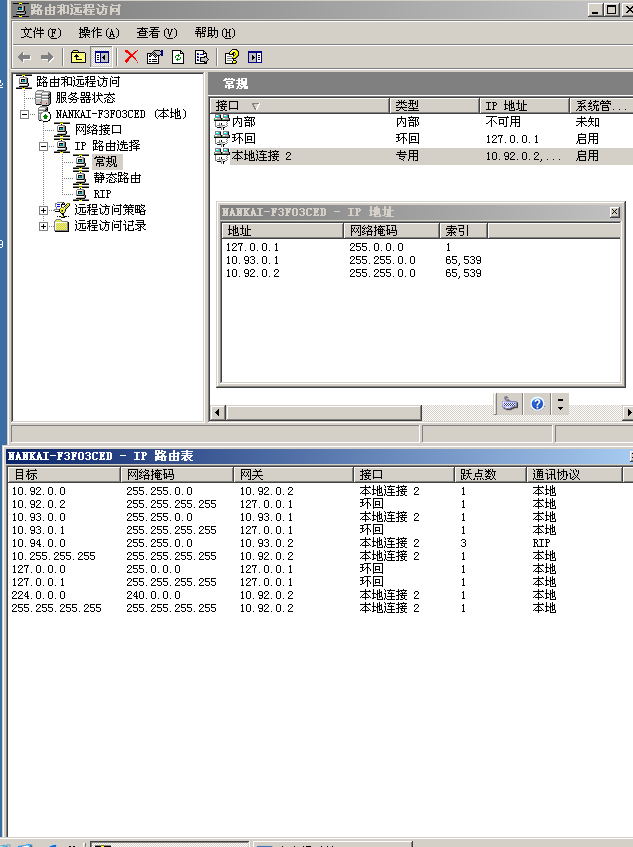
\includegraphics[width=0.6\textwidth]{rip22}
		\caption{R1添加到网络\text{10.94.0.0}的RIP路由\label{fig:rip1}}
	\end{minipage}
	\begin{minipage}[t]{0.48\textwidth}
		\centering
		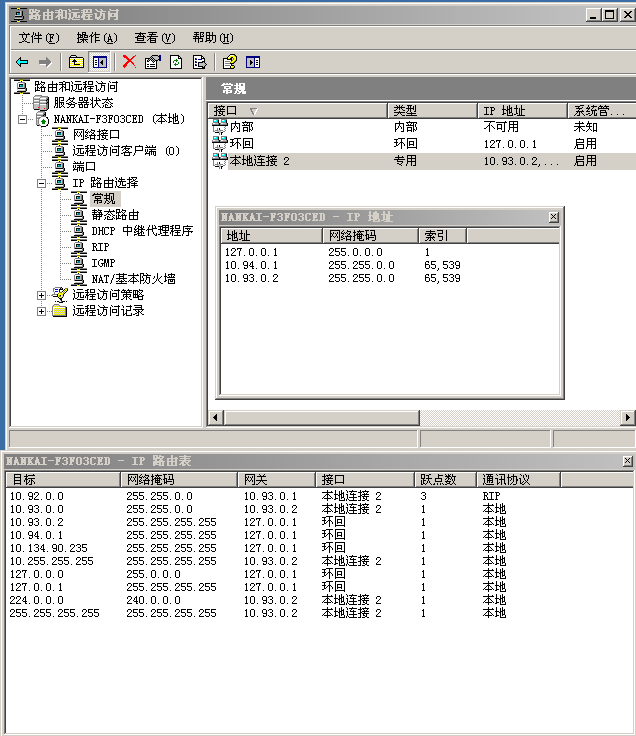
\includegraphics[width=0.68\textwidth]{riprouteandip3}
		\caption{R2添加到网络\text{10.92.0.0}的RIP路由 \label{fig:rip2}}
	\end{minipage}
\end{figure}

\subsubsection{连通性测试}
在配置好网络路由之后,需要对配置好的网络进行连通性测试,在本实验中,对任意两台机器之间均能够通过ping或者tracert命令正常连通,在下面主要展示主机A、B之间的连通性测试,测试结果如\figref{fig:A}、\figref{fig:B}所示(由于静态路由和RIP路由的结果没有区别在下面不做区分展示):
\begin{figure}[htbp]
	\begin{minipage}[t]{0.48\textwidth}
		\centering
		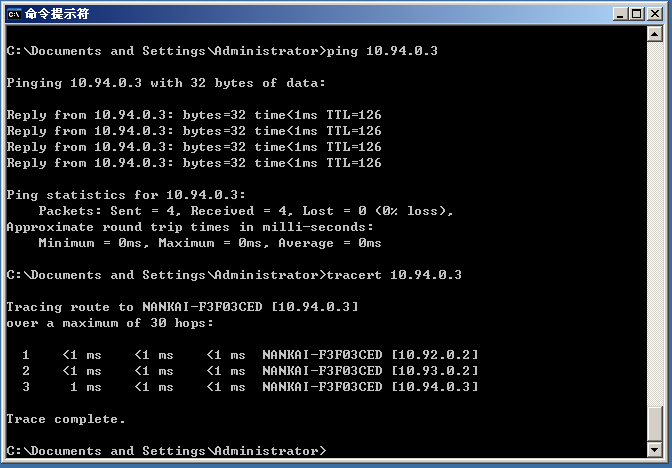
\includegraphics[width=0.7\textwidth]{s1t}
		\caption{主机Aping主机B结果截图\label{fig:A}}
	\end{minipage}
	\begin{minipage}[t]{0.48\textwidth}
		\centering
		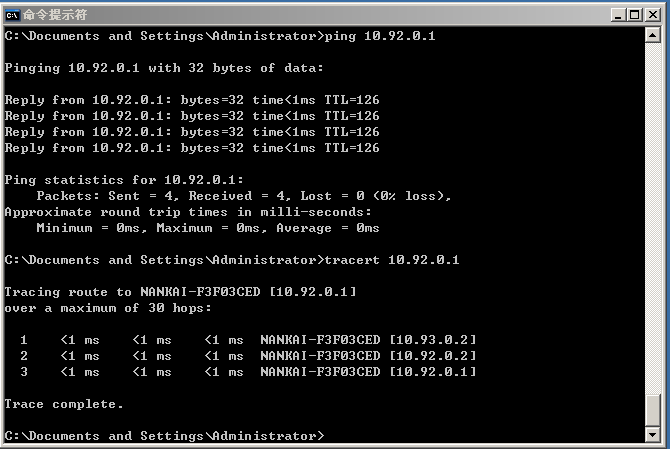
\includegraphics[width=0.78\textwidth]{s4tst}
		\caption{主机Bping主机A结果截图 \label{fig:B}}
	\end{minipage}
\end{figure}

\subsection{仿真环境路由配置}
\subsubsection{路由配置}
与虚拟机环境类似,仿真环境下的配置步骤基本没有区别,都是先进行IP地址的配置,然后配置静态路由或者动态RIP路由协议,\figref{fig:11}显示的是网络拓扑图以及相关接口的IP地址配置。
\begin{figure}[htbp]
	\centering
	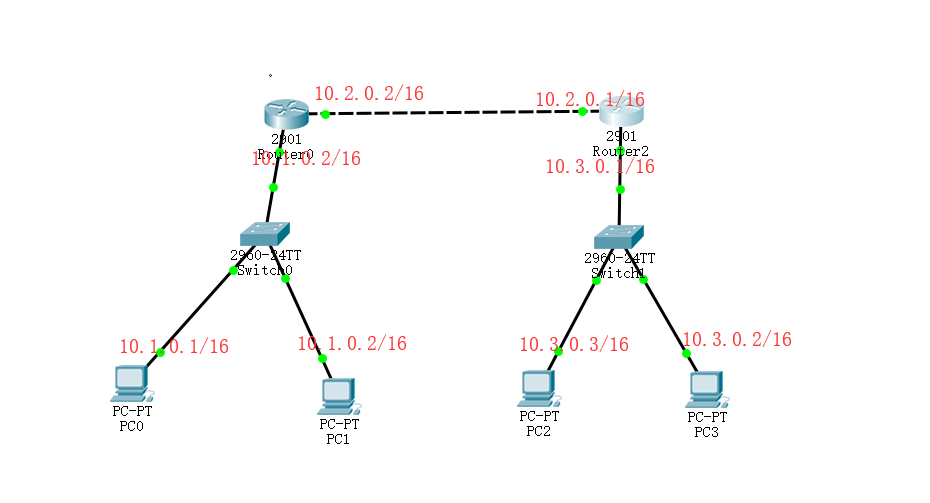
\includegraphics[width=0.6\textwidth]{网络拓扑图}
	\caption{仿真环境互联网拓扑图结构 \label{fig:11}}
\end{figure}
按照网络拓扑图中的IP地址配置好了主机的IP地址之后,进一步可以配置网络路由,在仿真环境下的路由配置主要通过路由器的CLI中的ip route 命令进行静态路由的配置,RIP路由配置通过router rip以及network 等命令实现,静态路由配置以及RIP路由配置的结果如\figref{fig:static}、\figref{fig:ripx}显示:
\begin{figure}[htbp]
	\begin{minipage}[t]{0.48\textwidth}
		\centering
		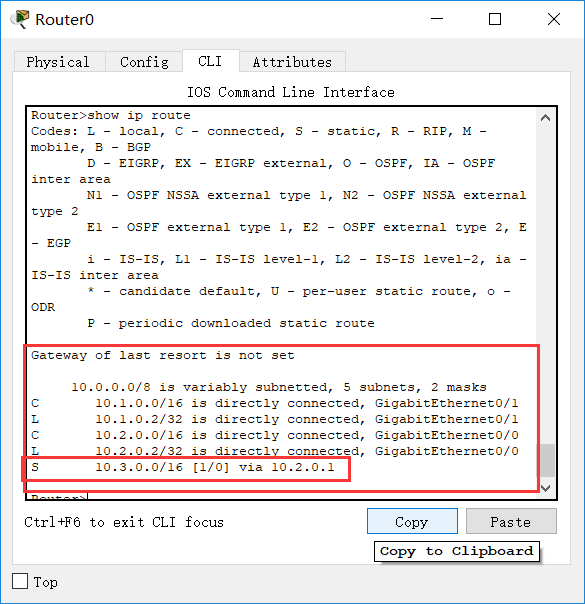
\includegraphics[width=0.7\textwidth]{staticroute1}
	\end{minipage}
	\begin{minipage}[t]{0.48\textwidth}
		\centering
		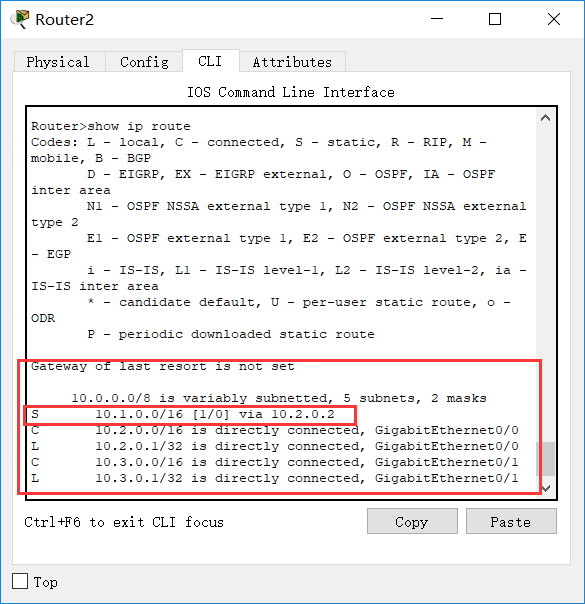
\includegraphics[width=0.78\textwidth]{staticroute2}
	\end{minipage}
	\caption{Static路由配置结果 \label{fig:static}}
\end{figure}

\begin{figure}[htbp]
	\begin{minipage}[t]{0.48\textwidth}
		\centering
		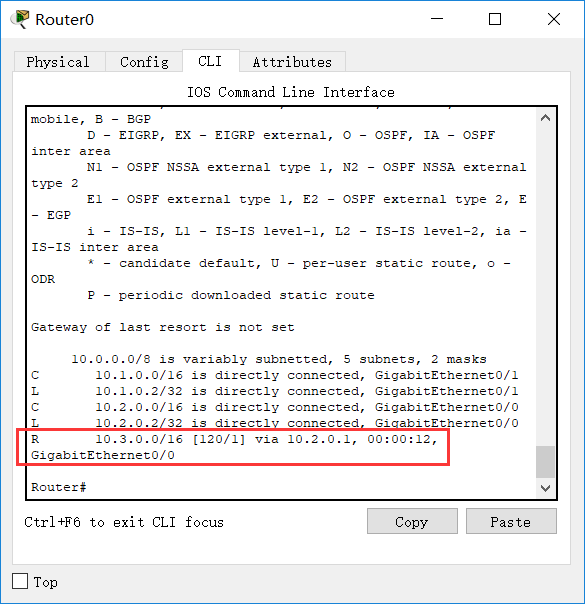
\includegraphics[width=0.7\textwidth]{rip1}
	\end{minipage}
	\begin{minipage}[t]{0.48\textwidth}
		\centering
		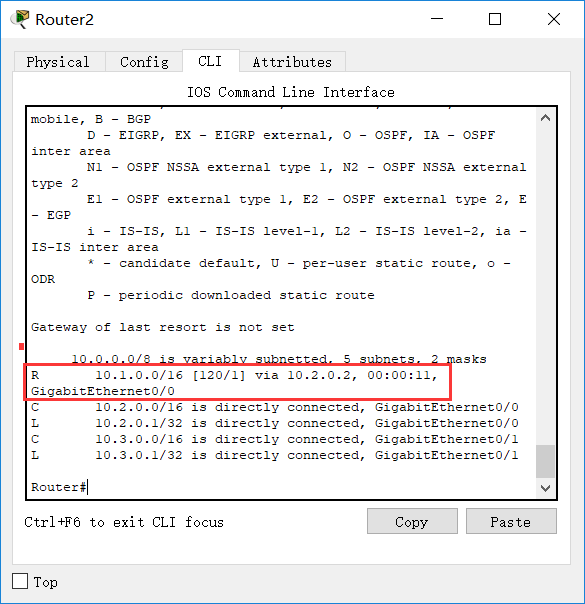
\includegraphics[width=0.78\textwidth]{rip2}
	\end{minipage}
\caption{RIP路由配置结果 \label{fig:ripx}}
\end{figure}
\subsubsection{连通性测试}
\begin{figure}[htbp]
	\begin{minipage}[t]{0.48\textwidth}
		\centering
		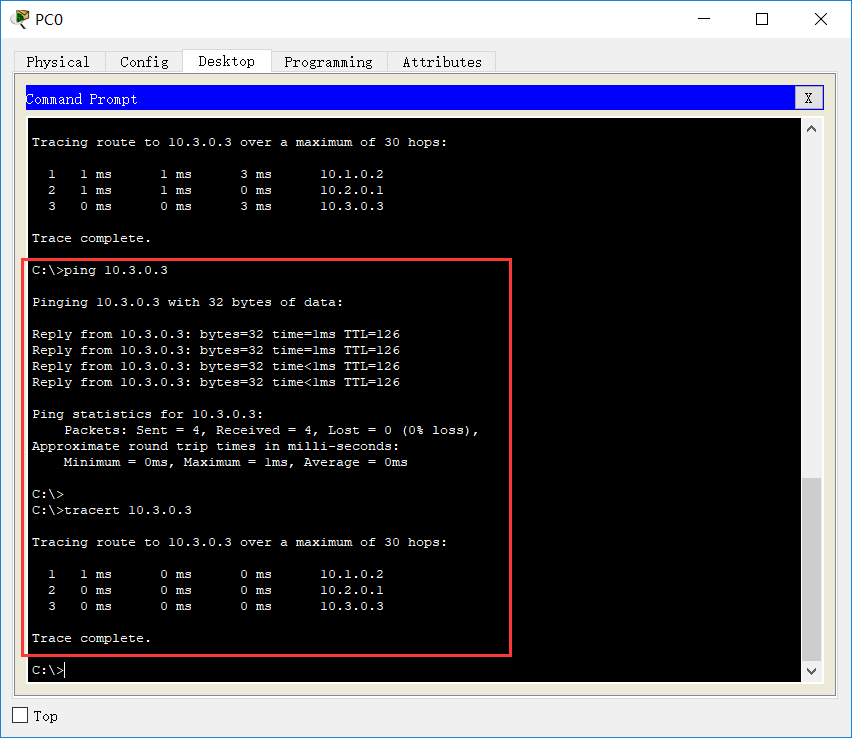
\includegraphics[width=0.7\textwidth]{riptest1}
	\end{minipage}
	\begin{minipage}[t]{0.48\textwidth}
		\centering
		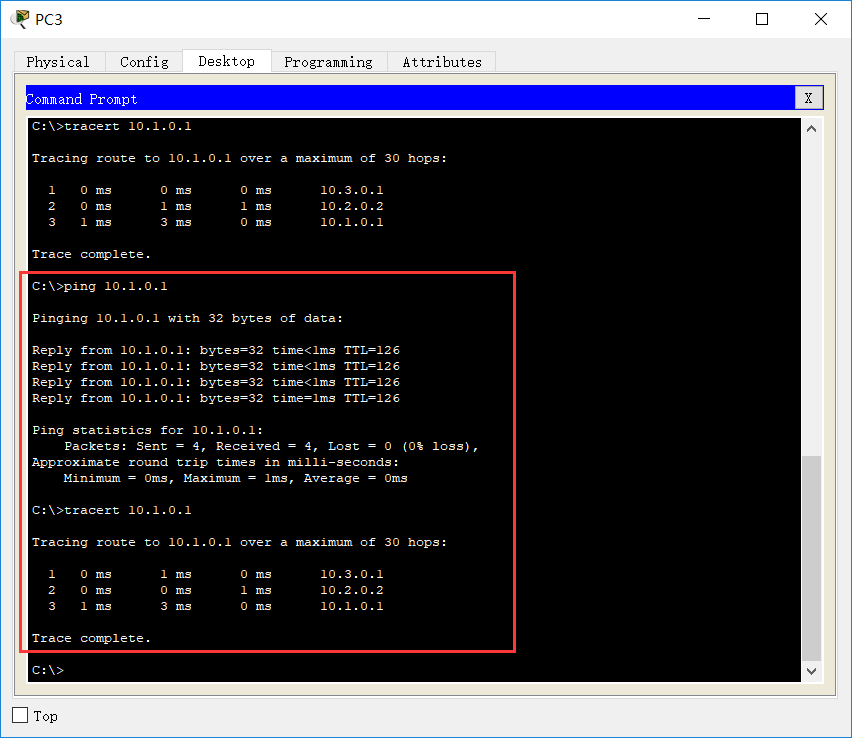
\includegraphics[width=0.78\textwidth]{riptest2}
	\end{minipage}
	\caption{连通性测试结果 \label{fig:test}}
\end{figure}

\subsubsection{数据包收发仿真演示}
数据包仿真收发的演示如\figref{fig:rip}所示,
\begin{figure}[htbp]
	\begin{minipage}[t]{0.48\textwidth}
		\centering
		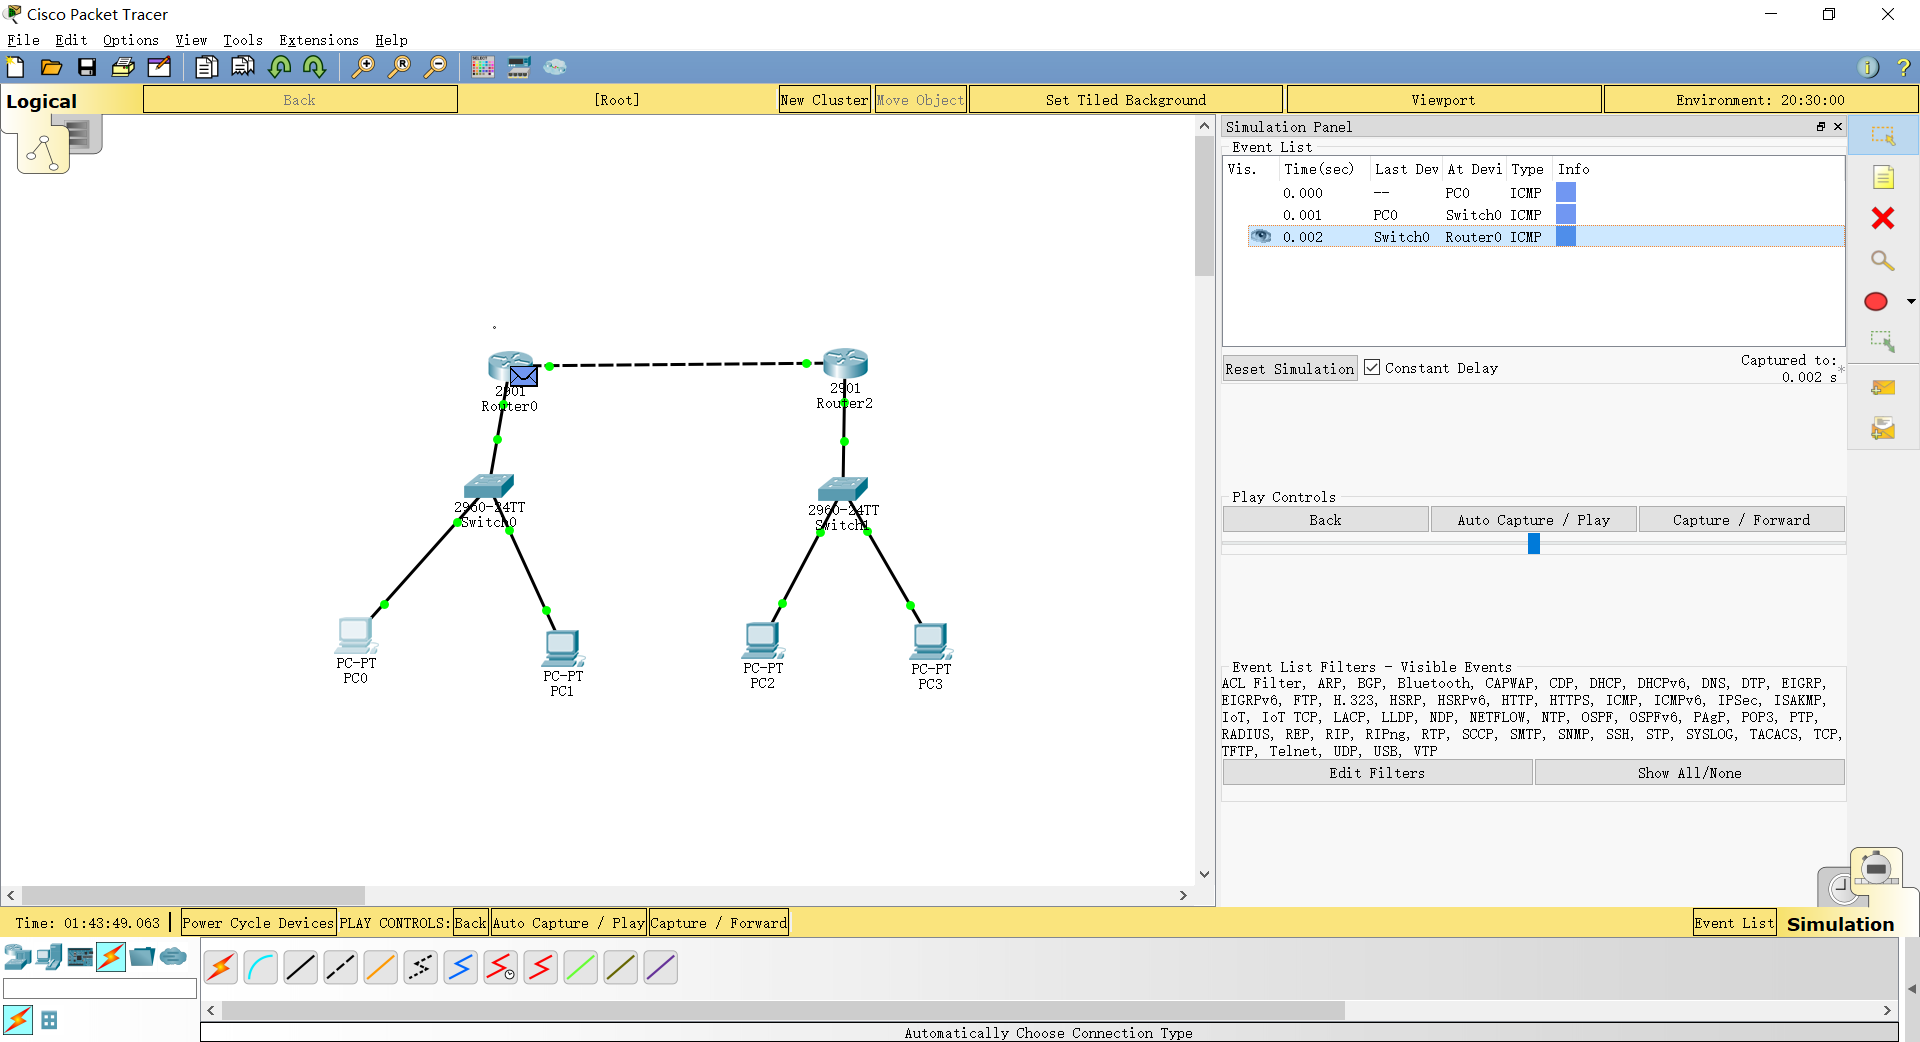
\includegraphics[width=0.7\textwidth]{simu1}
	\end{minipage}
	\begin{minipage}[t]{0.48\textwidth}
		\centering
		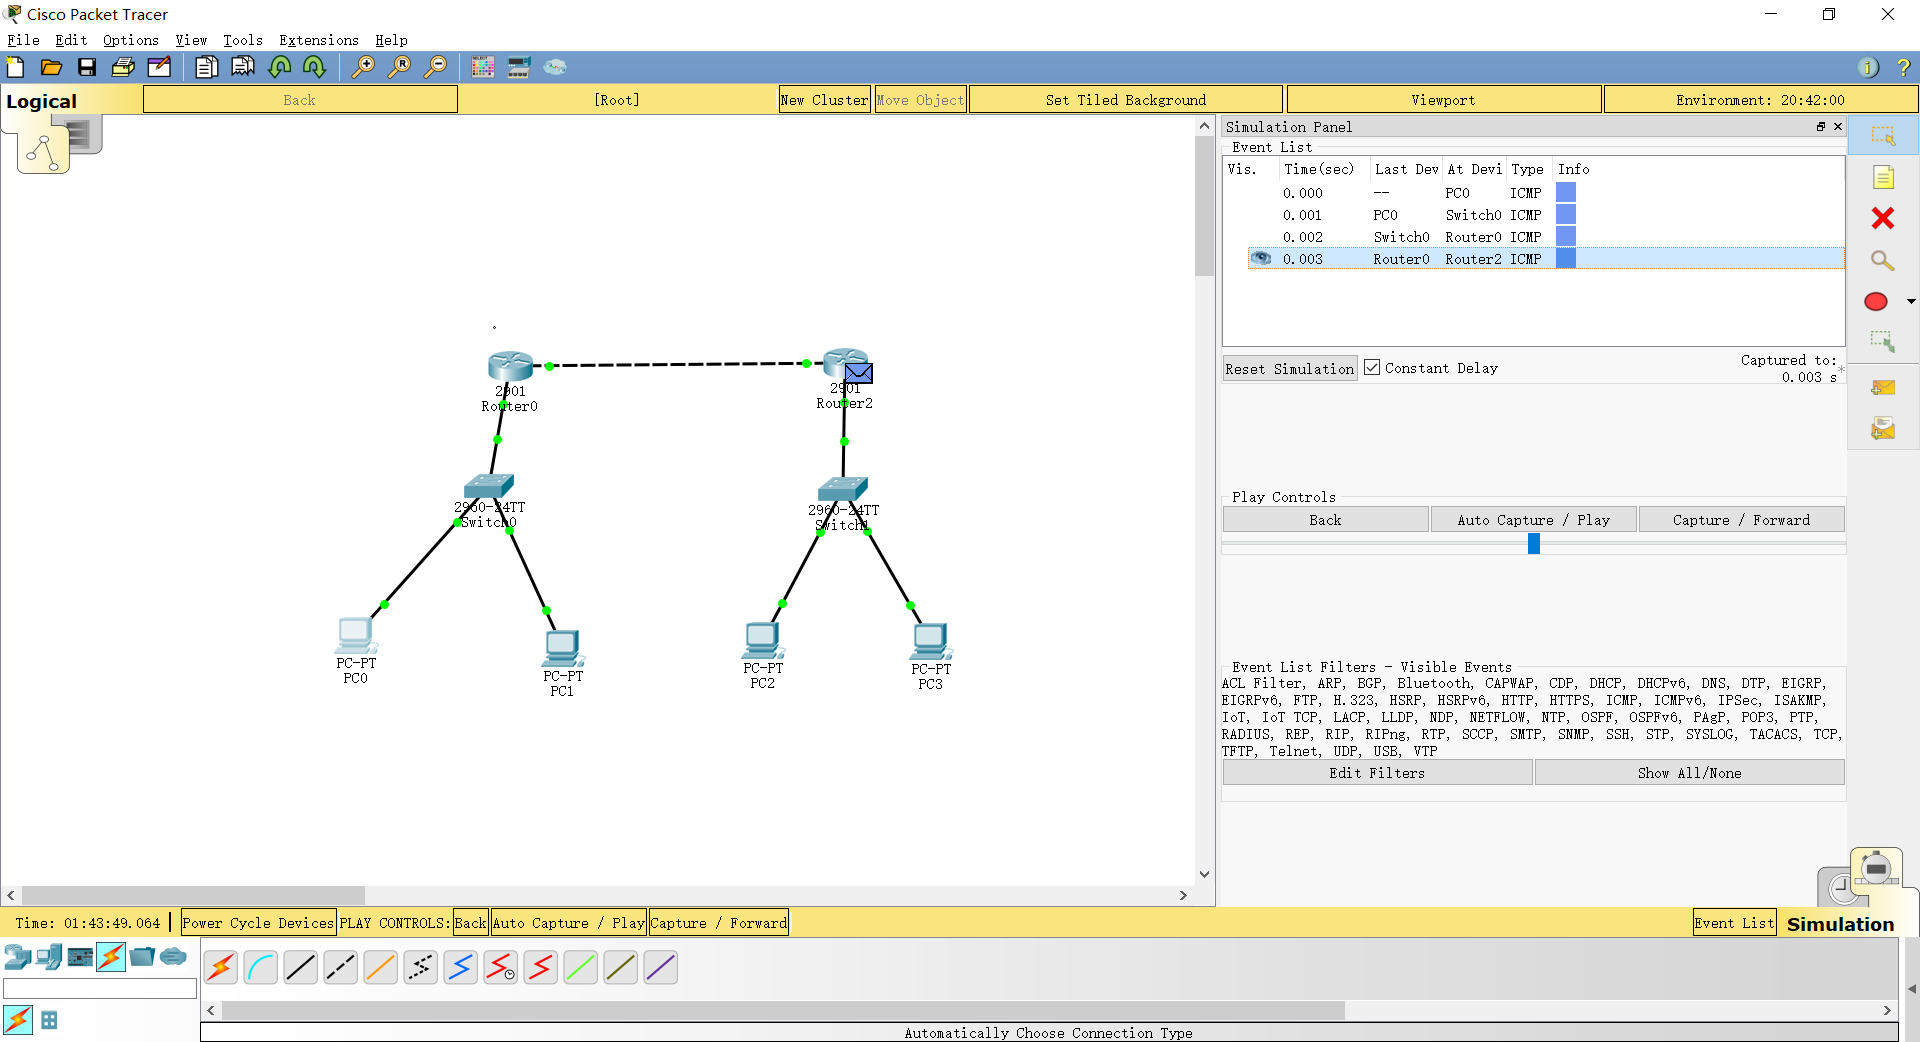
\includegraphics[width=0.78\textwidth]{simu2}
	\end{minipage}
	\begin{minipage}[t]{0.48\textwidth}
		\centering
		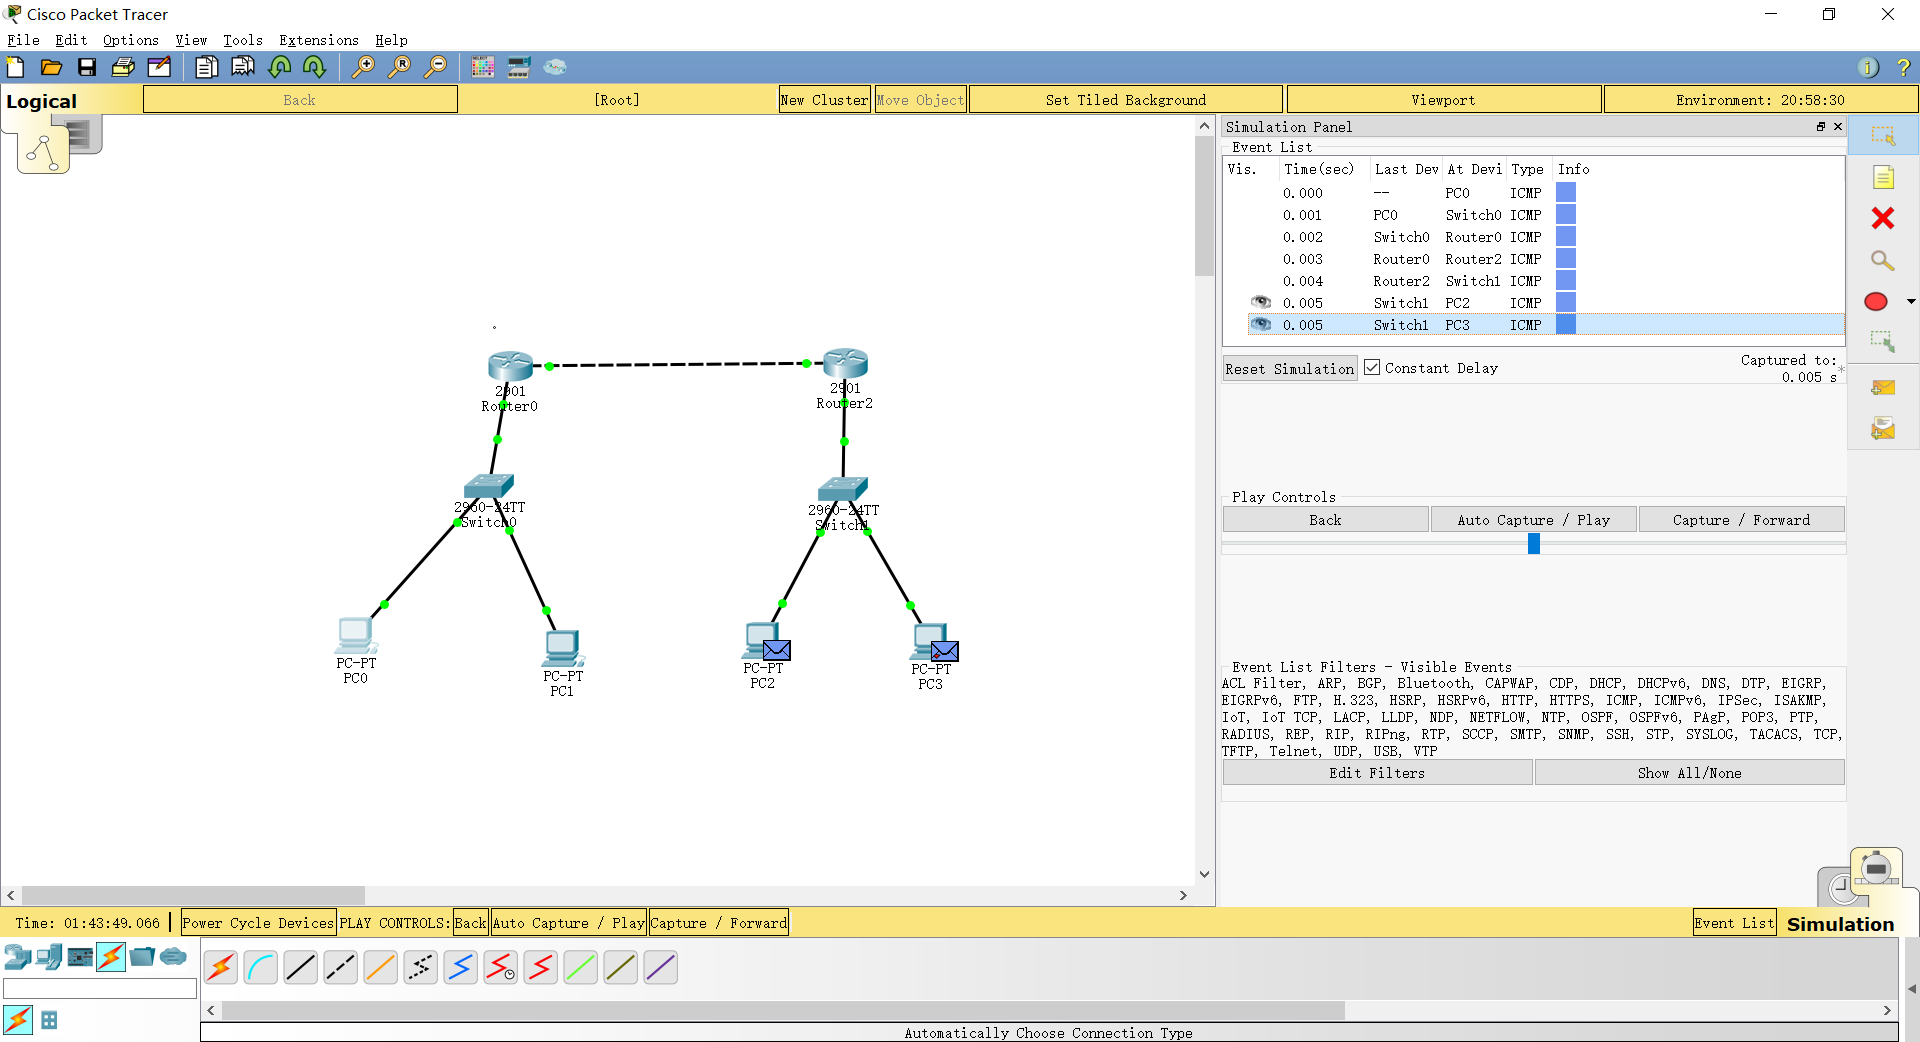
\includegraphics[width=0.7\textwidth]{simu4}
	\end{minipage}
	\begin{minipage}[t]{0.48\textwidth}
		\centering
		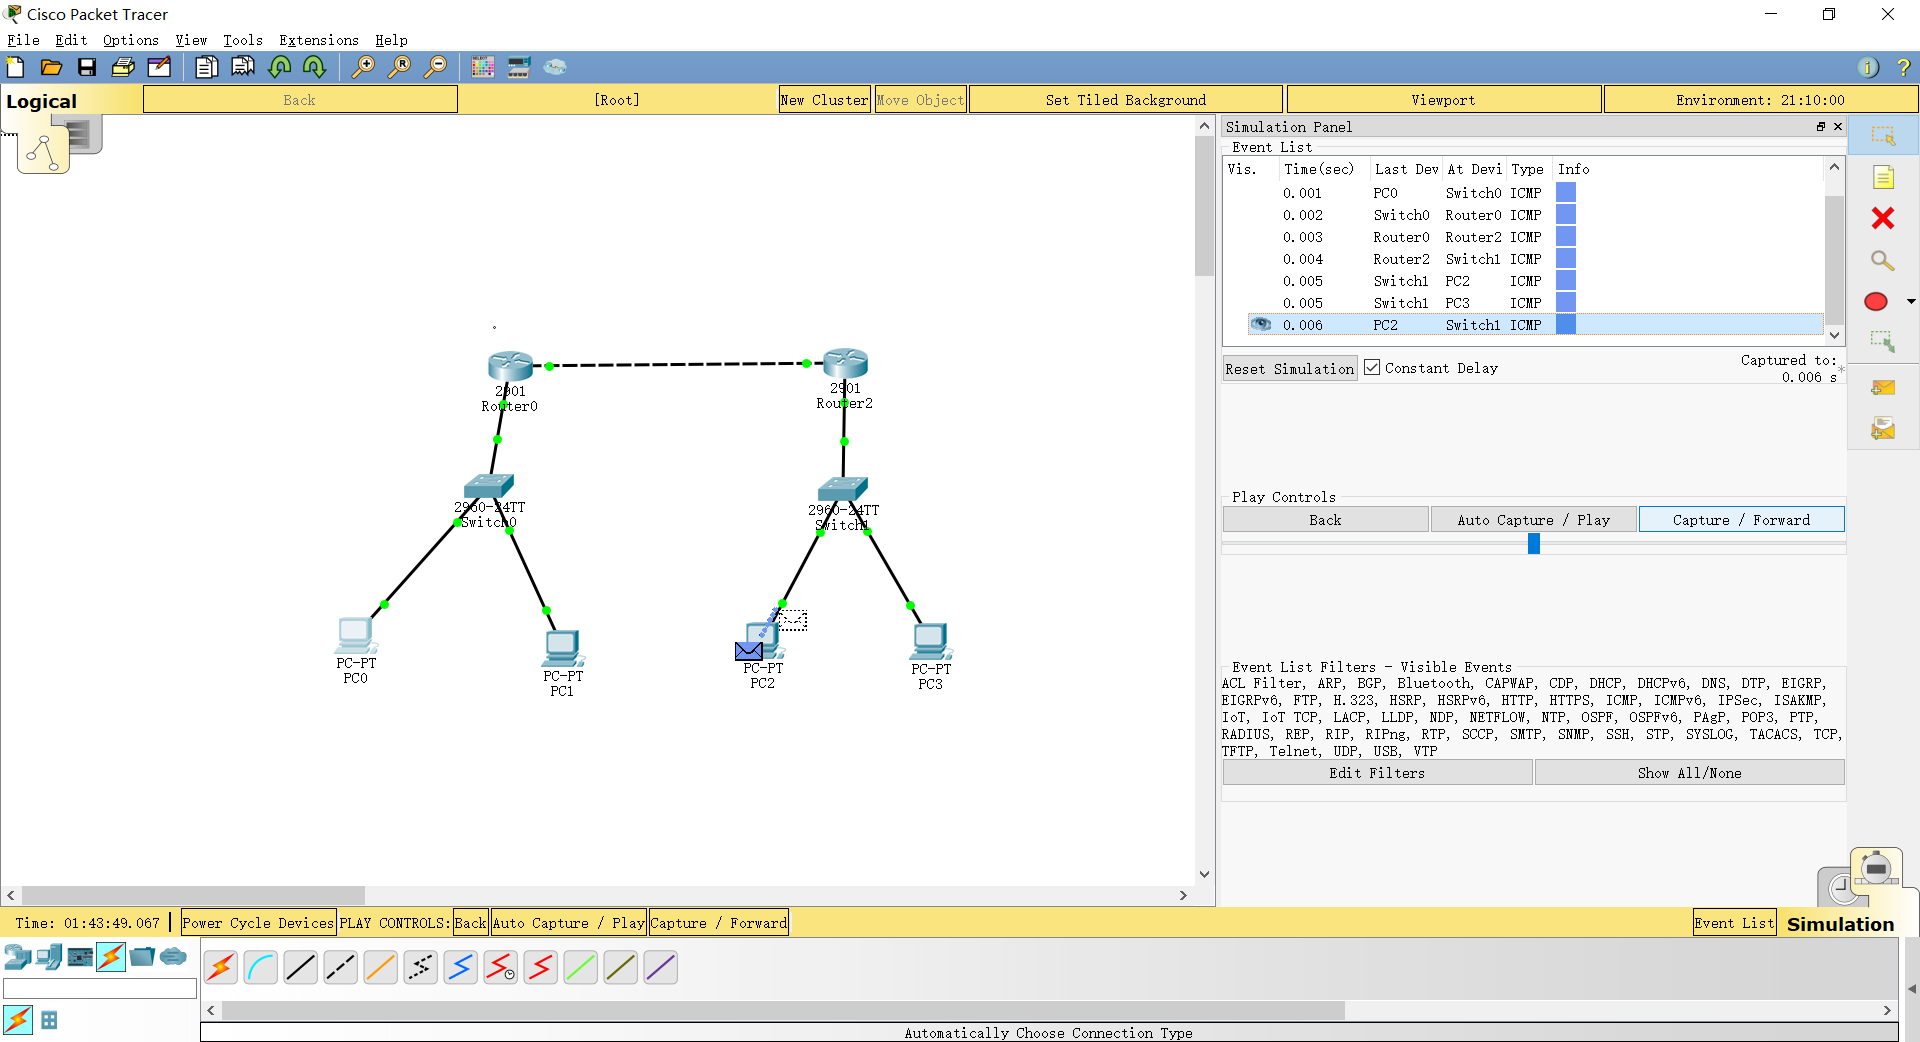
\includegraphics[width=0.78\textwidth]{simu5}
	\end{minipage}
	\begin{minipage}[t]{0.48\textwidth}
	\centering
	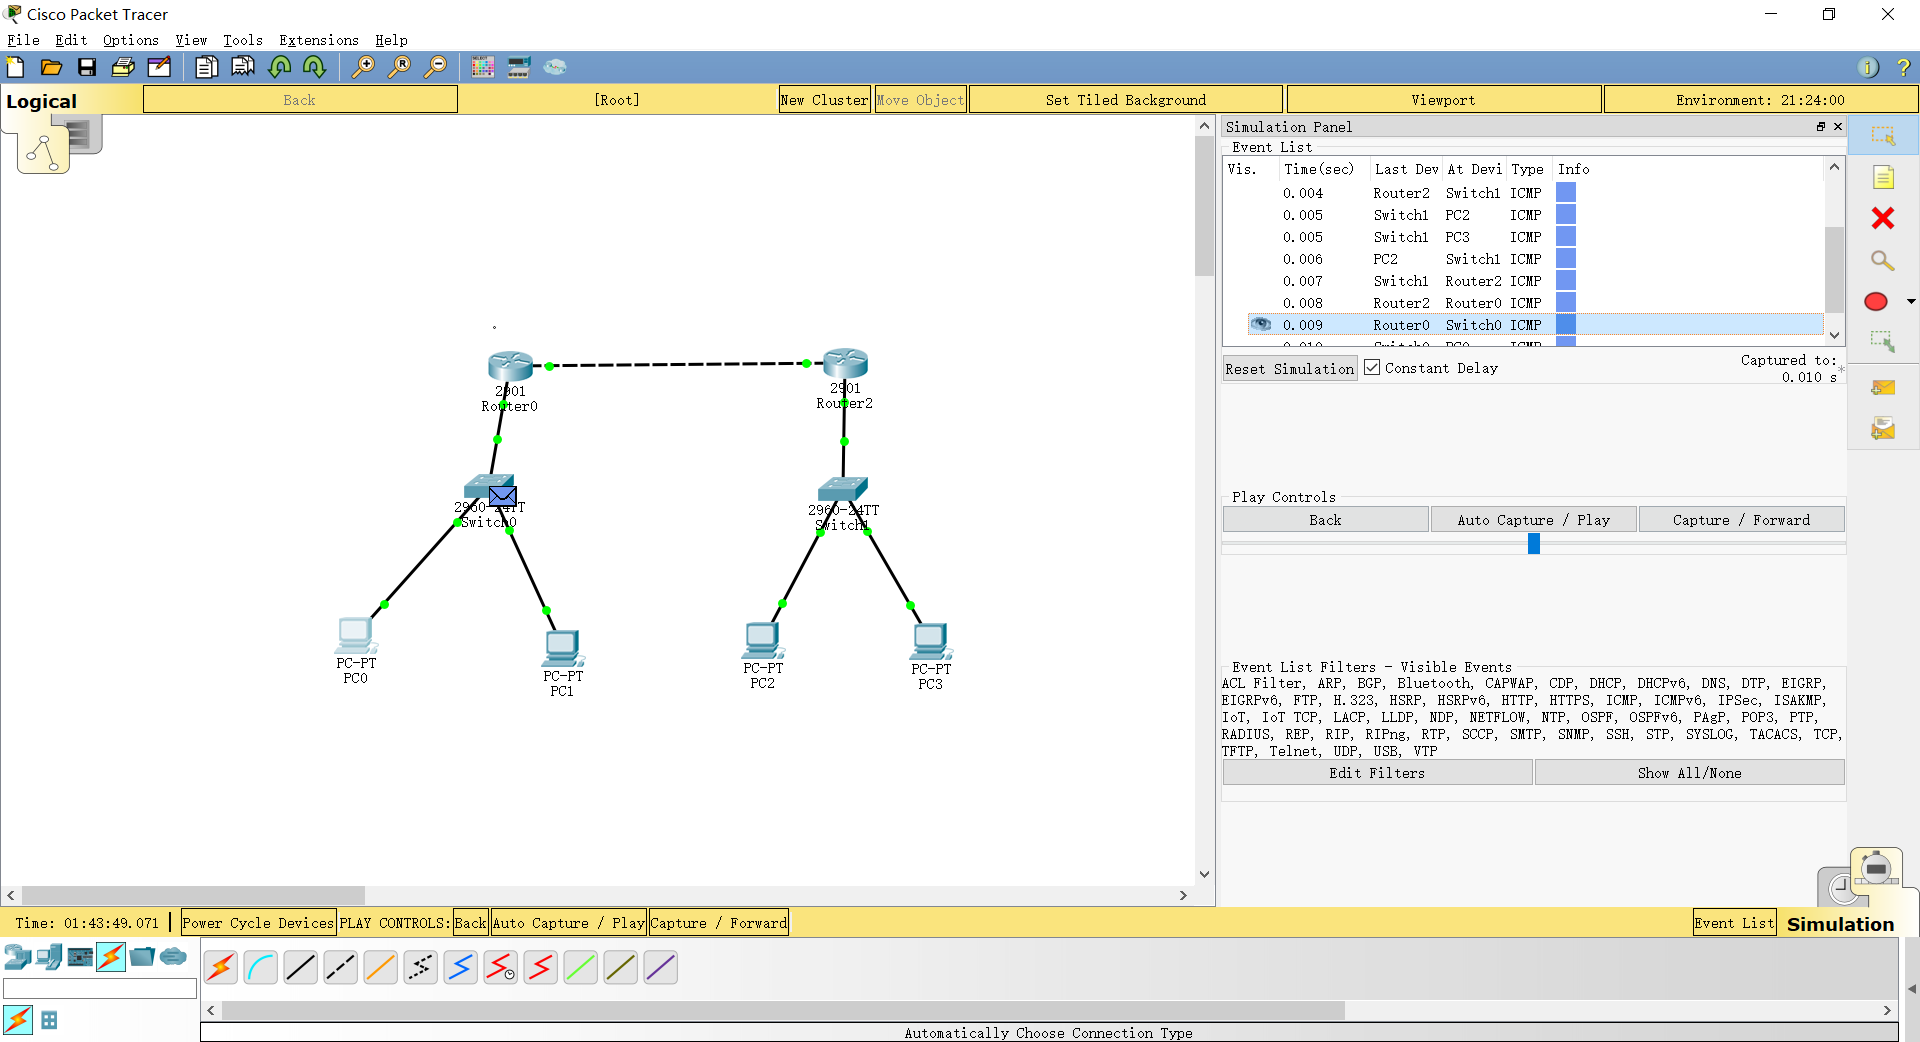
\includegraphics[width=0.7\textwidth]{simu6}
	\end{minipage}
	\begin{minipage}[t]{0.48\textwidth}
	\centering
	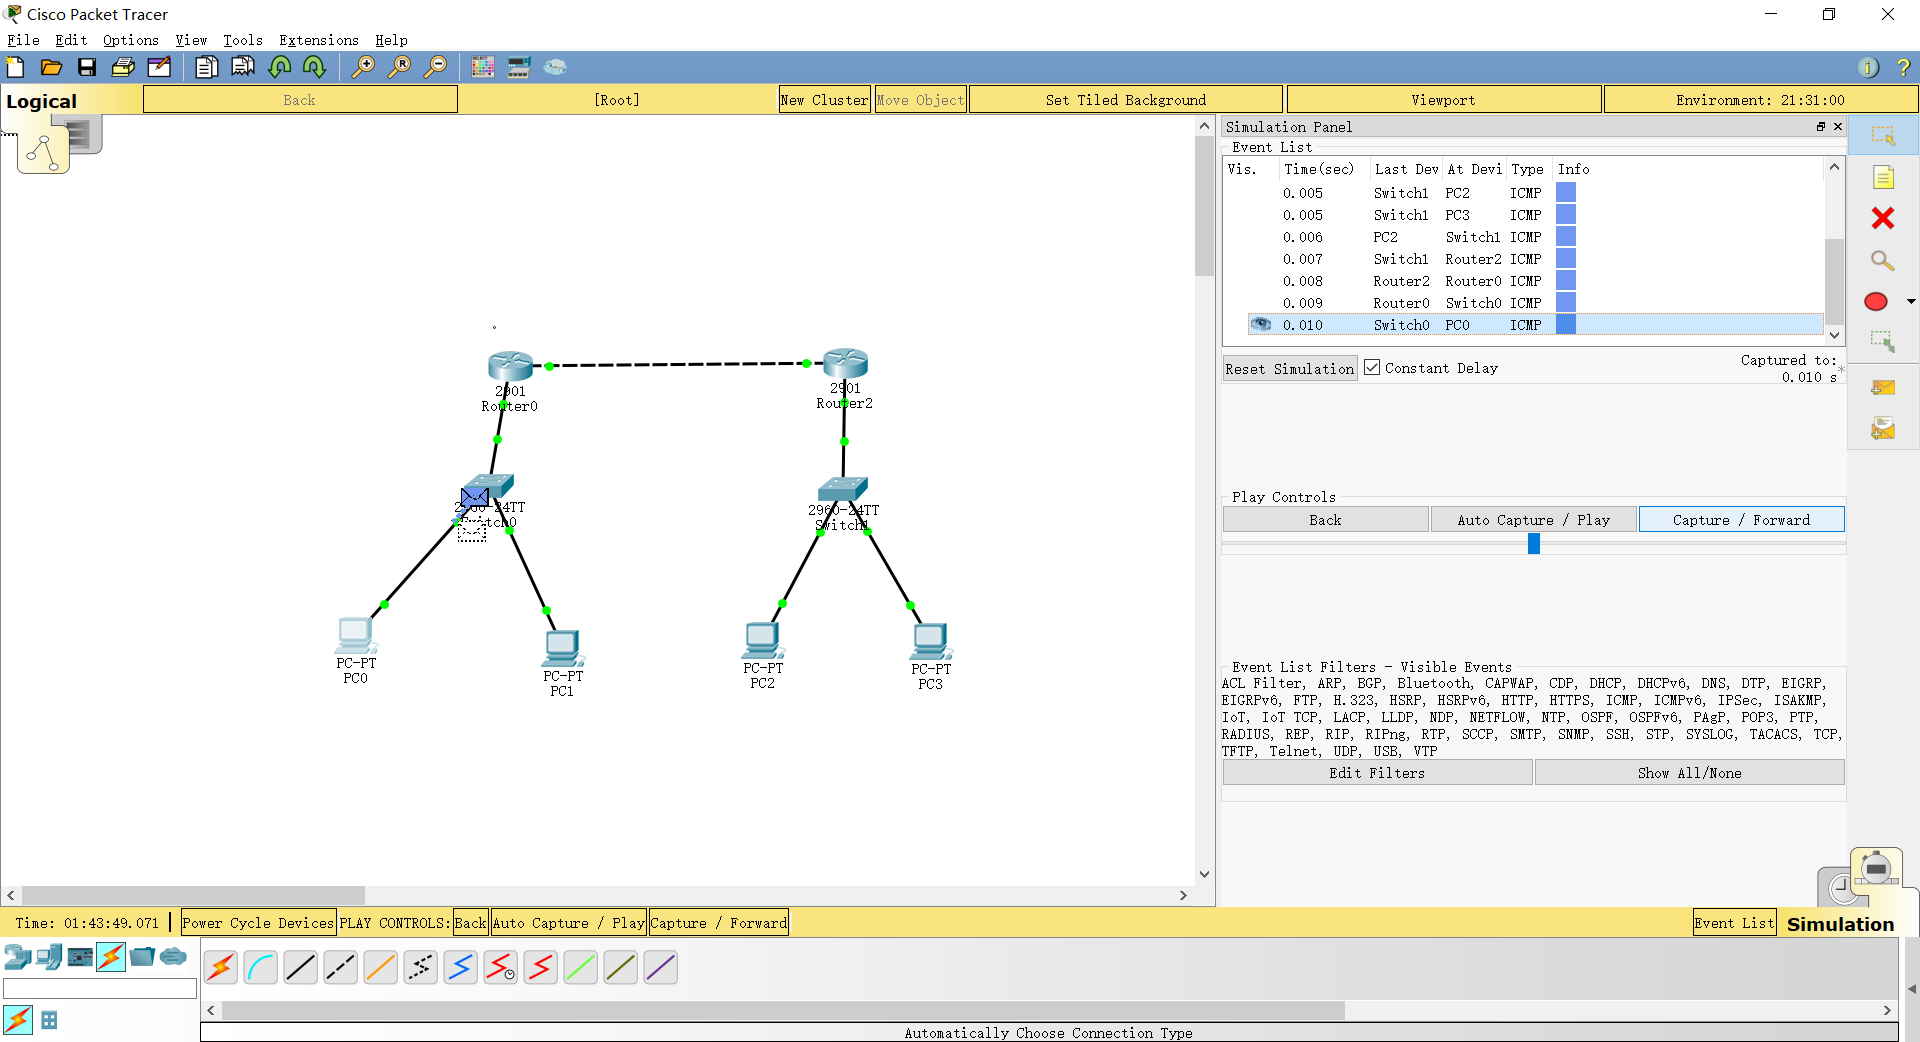
\includegraphics[width=0.78\textwidth]{simu7}
	\end{minipage}
	\caption{数据包收发过程演示 \label{fig:rip}}
\end{figure}
从图中的数据包收发过程能够看到,数据包通过发送端发出之后,通过交换机和路由器转到目的主机所在的物理网络,目的主机做出反馈之后通过之前的路径返回到目的主机,由于交换机和路由器都具有选择转发的功能所以在交换机2没有目的主机3的\text{MAC-IP}映射关系的时候是在所有的端口均进行转发的,但是在获取映射关系之后,就是针对性的数据包转发,因此响应数据包的回传是直接按照单一路径到达源主机的。

\section{总结与思考}
通过这次在四台虚拟机上进行网络路由的配置以及在仿真环境下配置路由并观察数据包的收发过程,进一步了解到了关于网络路由的相关知识,深入理解了路由器工作的基本原理和配置路由的相关工作,能够理解路由表形成的过程和路由表在网络通信中的巨大作用。虽然没有很快地完成所有的实验任务,但是最终在经过很多尝试后总算是成功了。在这次实验的过程中发现,实验室的机器还是会有一些不能理解的奇怪情况出现,之前没有及时完成就是有这方面的原因,换了几台机器后总算是把实验完成了。


% 如果想修改参考文献样式(非国标),请把下行取消注释,并换成合适的样式(比如 unsrt,plain 样式)。
%\bibliographystyle{aer}
%\bibliography{wpref}

\end{document}
